% NO NEED TO CHANGE ANYTHING IN THIS FIRST LINE
\documentclass[aps,prl,twocolumn,groupedaddress]{revtex4}

% INCLUDE PACKAGES

% -- THIS PACKAGE WILL LOAD GRAPHICS HANDLING FUNCTIONALITY
\usepackage{graphicx}
\usepackage{booktabs}

% DEFINE COMMANDS

% -- THIS COMMAND CREATES A SHORTHAND FOR \begin{equation}
\newcommand{\beq}{\begin{equation}}
% -- THIS COMMAND CREATES A SHORTHAND FOR \end{equation}
\newcommand{\eeq}{\end{equation}}
% -- THIS COMMAND TAKES ONE ARGUMENT AND PLACES IT INSIDE OF PARENTHESIS
\newcommand{\of}[1]{\left(#1\right)}

\begin{document}


\title{Determining maximum power output of cantilever based Piezoelectric Energy Harvester under various resonant conditions}


\author{Kurt VonEhr}
\email[]{vonehrk@gvsu.edu}
\affiliation{ Padnos College of Engineering and Computing, Grand Valley State University}

\date{\today}

\begin{abstract}

Piezoelectric devices will produce varying outputs (voltage, current, etc) depending on the resonance of their structure. For this experiment, the structure under study will be a single bimorph piezocantilever containing a steel sheet metal substrate. Without performing a complex mathematical analysis of the systmem, a rough optimization of a piezoelectric cantilever harvesting system can be obtained through experimentation. In this experiment, the maximum power output of the energy harvesting device will be determined by measuring the charge accumlated on a storage capacitor of known capacitance, after a consistent number of plucks and pluck angle for each particular resonant configuration. The resonsance will be varied by moving a tip mass to different positions along the cantilever arm. The cantilever substrate will be assumed to be massless with respect to the tip mass. The results should illustrate which length will maximize the power output of the cantilever arm when plucked. This experimentation is necessary in order to prototype design a roughly optimized Harvesting Node Device (HND). This device will contain 12 cantilever harvesting arms and be used to transmit data. The HND is the driving motivation of this experiment. 
\end{abstract}
 
\maketitle

\section{Procedure}
\subsection{Setup}

Due to the unique structure of the desired HND (not in the scope of this report), a non commercially available piezo cantilever device must be constructed. A piezo sheet of size 2.85in x 2.85in was purchased and is the starting point for the piezo dimension choices. The design of the HDN will include 12 bimorph cantilevers. To optimize the available piezo material for 12 cantilevers,  the dimensions of each bimorph structure will be as shown in FIG. 1. The values of X1 and X2 shown in FIG. 1, will be varied individually, such that the particular lengths can be isolated and the associated generated charge measured. To ensure that the generated power is consistant, the angle of the pluck release will be held constant. The angle will be loosely based upon the commercial product manufactered by Volture, who lists a maximum tip to tip displacement of .12in for the V22BL model \footnotemark\footnotetext{\url{http://www.mide.com/pdfs/Volture_Datasheet_001.pdf}}. The distance from base to tip is 2.75in. The angle of displacement is therefore: 

\begin{equation}
 2.49 ^\circ = \arctan (.12/2.75)
\end{equation}

\begin{figure}[ht!]
  \centering
  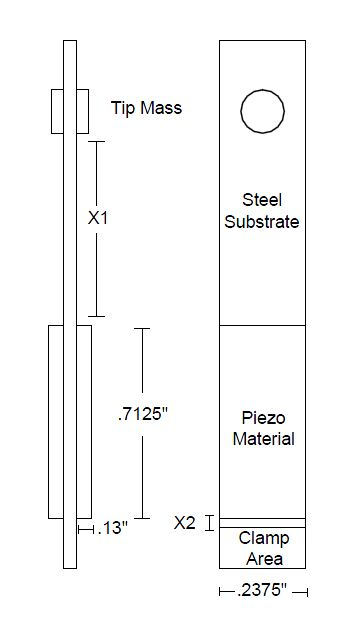
\includegraphics[scale=0.6]{Bimorph_Cantilever.jpg}
  \caption{Laboratory Test Bimorph Piezoelectric Cantilever}
\end{figure}

Using this angle (1) as a reference and prior knowledge of the bimorph cantilever, an angle of $3^\circ$ is used. In previous experiments, the cantilever was allowed to bend further than $2.5^\circ$ without damage. 

The sheet was cut by razo blade etching and a controlled break as suggested on this webpage: \url{http://www.piezo.com/tech3faq.html}. The piezo material will then be secured to the steel substrate using a dielectric epoxy. The bulk steel substrate that was used, was 25 gage shim stock. The piece was cut to the dimensions of FIG. 1. The procedure to create a parallel, double current configuration, as illustrated in FIG. 2 is as follows. 1.) Mark the piezo sheet stock on one side before cutting into two peices. This is imporant because the material is polarized, and to create the double current configuration, both piezo components of the bimorph must face in the same direction 2.) After cutting the shim stock to the desired size, remove any rust or debris from the surface. This will allow for the epoxy to adhere to the surface, as well as conduct with a lower resistance. 3.)Tape the shim stock to the table and mark the location of one end of the piezo component, as well as the ends of the shim stock on the table. This will allow both sides to have the piezo component located in the same position. The epoxy will cover up marks on the shim stock substrate. 4.) After mixing the epoxy, spread a thin layer onto the shim stock substrate. 5.) Quickly, before the epoxy begins to set, take a piece of tape and fold it so that the piezo component can be picked up and placed onto the epoxy without touching the epoxy or getting epoxy onto both sides of the piezo component. Be sure that the piezo component is placed exactly where it should be, so that it is not necessary to slide the piece around on the epoxy. If the piece is slid around, the epoxy will ride up the side of the piezo component and onto the outward facing surface. It is critical that this not occur, otherwise harvesting will be severely limited due to a short between both sides of the piezo component.

\begin{figure}[ht!]
  \centering
  \includegraphics[scale=0.6]{BNact1.jpg}
  \caption{Bimorph Cantilever Configurations}
\end{figure}

\subsection{Experiment}
  
The purpose of this experiment is to determine the best clamp position for the cantilever base and the length of the substrate. This is determined experimentally by varying each parameter individually and measuring the voltage on the storage capacitor after 20 plucks at an angle of $3^\circ$. To keep the design as compact as possible, the substrate material will have a maximum length of 2''. 

\section{Results}

asdf

\begin{table}[htbp]
  \centering
  \caption{Add caption}
    \begin{tabular}{rrr}
    \toprule
    \textbf{Vin} & \textbf{Vc} & \textbf{Ve} \\
    \midrule
    X     &  X   & X  \\

    \bottomrule
    \end{tabular}%
  \label{tab:addlabel}%
\end{table}%






% THE FINAL SECTION IS DISCUSSION
\section{Discussion}

\vfill


\end{document}
%
% ****** End of file template.aps ******
